\documentclass[12pt]{report}
\usepackage[print,nopanel]{pdfscreen}
%\begin{print}
\usepackage{mathptmx}% http://ctan.org/pkg/mathptmx
\usepackage{mathptmx}% http://ctan.org/pkg/mathptmx
%\section{type}
\usepackage{lastpage}
\usepackage{macro/macro}
\usepackage{float}
\usepackage{wrapfig}
\usepackage{fancyhdr}
\usepackage{verbatim}
\bibliographystyle{IEEEtranN}
%Options: Sonny, Lenny, Glenn, Conny, Rejne, Bjarne, Bjornstrup
\usepackage[Glenn]{fncychap}
\lhead{\large\bfseries}
\usepackage[left=3.5cm, right=1.25cm, top=2.5cm, bottom=1.25cm]{geometry}
\pagestyle{fancy}
%\end{print}
\margins{.5cm}{.5cm}{.5cm}{.5cm}
\begin{screen}

\renewcommand{\encodingdefault}{T1}
\usepackage{setspace}
\linespread{1.5}
\renewcommand{\rmdefault}{ptm}
\end{screen}
\screensize{8cm}{9cm}
\overlay{overlay8.pdf}
\usepackage{graphicx}


\begin{document}
\newcommand{\centertext}[1]{\begin{center}\textbf{#1}\end{center}}
\newcommand{\student}{\vskip 2.5cm}
\newcommand{\supervisor}{\vskip 2cm}
\newcommand{\stamp}{\vskip 2.5cm}
\newcommand{\HRule}{\rule{\linewidth}{0.5mm}}
\newcommand{\projecttitle}{\Huge \bf{Analyzing OSM data and Graphing using GraphX}\vskip 0.2in}
\newcommand{\tab}[1]{\hspace{.4\textwidth}\rlap{#1}}
\newcommand{\itab}[1]{\hspace{.05\textwidth}\rlap{#1}}
\newcommand{\logo}[1]{\includegraphics[scale=0.7]{#1}}
\newcommand{\submitted}{
\vskip 0.1in
\textnormal{Submitted for partial fulfilment of the Degree\\
of\\
Bachelor of Technology\\
(Computer Science)\\
}
\vskip 1 cm
\begin{figure}[!ht]
\centering

\includegraphics[width=0.3\textwidth]{input/images/gne.jpg}                   
\hspace{-1.5em}
\end{figure}
%\image{0.7}{images/gne.jpg}{}

\vskip 0.5cm
\begin{minipage}{0.4\textwidth}
\begin{flushleft} \large
{Submitted By:}\\
\textnormal{Sharanmeet Singh\\
1410926}\\ 
\textnormal{Ranvir Singh\\
1410917} 
\end{flushleft}
\end{minipage}
~
\begin{minipage}{0.4\textwidth}
\begin{flushright} \large
{Submitted To:} \\
\textnormal{Sukhjit Singh Sehra\\ Training Coordinator\\ CSE Department                                                                                   } % Supervisor's Name
\end{flushright}
\end{minipage}\\[2cm]
\HRule \\[0.4cm]
\textnormal{Department of Computer Science \& Engineering \\
Guru Nanak Dev Engineering College \\
Ludhiana 141006}
}
\newcommand{\pagetitle}{\begin{center}
\projecttitle
\Large\textbf{}\\
\submitted
\vskip 0.2cm

\end{center}}
\newcommand{\openoffice}{\textbf{OpenOffice}}
\newcommand{\frontmatter}[1]{\begin{Large} \textbf{#1} \end{Large}}
\newcommand{\ppttitle}{\begin{center}
\end{center}}






\begin{screen}
\ppttitle
\end{screen}
\footskip 0.7cm
\thispagestyle{empty} 
\pagetitle
\newpage
\pagenumbering{Roman}
\cfoot{\thepage}

\begin{center}
{\Huge \noindent \bf{Acknowledgement}\vskip 0.2in}
\end{center}
 \hrulefill \\

We, students of Guru Nanak Dev Engineering College, Ludhiana, have taken efforts in this project.
However, it would not have been possible without the kind support and help of many individuals
and organizations. I would like to extend my sincere thanks to all of them.\\

The author is highly grateful to Dr. M.S. Saini Director, Guru Nanak Dev Engineering College, Ludhiana for providing her with the opportunity to carry out his Major Project in this estimed college, Guru Nanak Dev Engineering College, Ludhiana.\\

The author would like to whole heartedly thank Dr. Sukhjit Singh Sehra, Training Coordinator, CSE department, Guru Nanak Dev Engineering College, Ludhiana who is a vast sea of knowledge and without whose constant and never ending support and motivation, it would never have been possible to complete the project and other assignments so efficiently and effectively.\\

Finally, I would like to thank all the organisations and indivisuals who created such great tools and algorithms and helped us to complete the project. 

\vskip 1.0cm 
\noindent Ranvir Singh
\vskip 1.0cm 
\noindent Sharanmeet Singh




\newpage

\begin{center}
{\Huge \bf{Abstract}\vskip 0.2in}
\end{center}
 \hrulefill \\

This is a research based project in which we have compared the processing time of various algorithms using apache spark and traditional serial programming on various data sets. As the size of the data sets changes, the difference in the processing time changes, producing some great results.\\\\
In this project we have used two systems one is the osmnx which is the traditional serial system in python. This uses simple serial programs to create the graphs. With small data sets the OSMnx creates the graphs faster.\\\\
On the other hand apache spark is used to create graph using the parrallel processing power of python program. With larger data sets the graph is created in lesser time.\\\\
GraphFrame is a spark API which takes data frame as input and created graphs so that we run parrallel programs using python.\\\\
Code related to this project is open source and shared using GitHub.




\newpage
\tableofcontents
\newpage
\listoffigures

\newpage

\pagenumbering{arabic}
\cfoot{\thepage}

\newpage
\chapter{Introduction To Organisation}

\begin{figure}[ht]
\centering
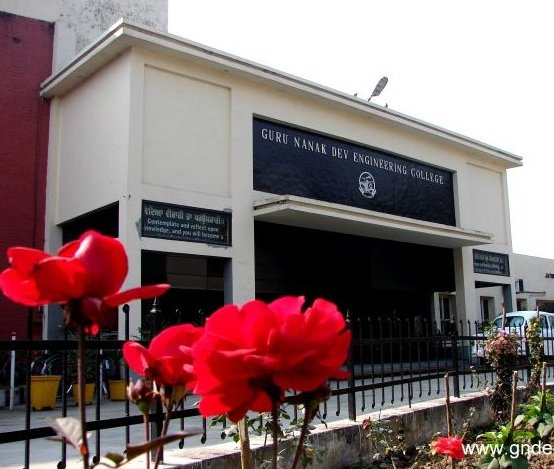
\includegraphics[scale=0.5]{input/images/gndec.jpg}
\caption{Guru Nanak Dev Engineering College}
\end{figure}
\hspace{-1.7em}
 Guru Nanak Dev Engineering College was established by the Nankana Sahib Education Trust Ludhiana. The Nankana Sahib Education Trust i.e NSET
was founded in memory of the most sacred temple of Sri Nankana Sahib, birth place
of Sri Guru Nanak Dev Ji. With the mission of Removal of Economic Backwardness
through Technology Shiromani Gurudwara Parbandhak Committee i.e SGPC started a
Poly technical was started in 1953 and Guru Nanak Dev Engineering College was established in 1956.\\
NSET resolved to uplift Rural areas by admitting 70\% 
of students from these rural
areas ever year. This commitment was made to nation on 8th April, 1956, the day
foundation stone of the college building was laid by Dr. Rajendra Prasad Ji, the First
President of India. The College is now ISO 9001:2000 certified.\\
Guru Nanak Dev Engineering College campus is spread over 88 acres of prime land
about 5 Kms from Bus Stand and 8 Kms from Ludhiana Railway Station on Ludhiana-Malerkotla Road. The college campus is well planned with beautifully laid out tree plantation, pathways, flowerbeds besides the well maintained sprawling lawns all around. It
has beautiful building for College,Hostels,Swimming Pool,Sports and Gymnasium Hall
Complex, Gurudwara Sahib, Bank, Dispensary, Post Office etc. There are two hostels
for boys and one for girls with total accommodation of about 550 students. The main
goal of this institute is:\\
\begin{itemize}
\item To build and promote teams of experts in the upcoming specialisations.
\item To promote quality research and undertake research projects keeping in view their relevance to needs and requirements of technology in local industry.
\item To achieve total financial independence.
\item To start online transfer of knowledge in appropriate technology by means of establishing multipurpose resource centres.
\end{itemize}



\newpage
\chapter{Introduction to Project}
\section{Overview}
\subsection{What is OSM?}
OpenStreetMap (OSM) is a collaborative project to create a free editable map of the world. The creation and growth of OSM has been motivated by restrictions on use or availability of map information across much of the world, and the advent of inexpensive portable satellite navigation devices. OSM is considered a prominent example of volunteered geographic information.\\

Created by Steve Coast in the UK in 2004, it was inspired by the success of Wikipedia and the predominance of proprietary map data in the UK and elsewhere. Since then, it has grown to over 2 million registered users, who can collect data using manual survey, GPS devices, aerial photography, and other free sources. This crowdsourced data is then made available under the Open Database Licence. The site is supported by the OpenStreetMap Foundation, a non-profit organisation registered in England and Wales.\\

Rather than the map itself, the data generated by the OpenStreetMap project is considered its primary output. The data is then available for use in both traditional applications, like its usage by Craigslist, OsmAnd, Geocaching, MapQuest Open, JMP statistical software, and Foursquare to replace Google Maps, and more unusual roles like replacing the default data included with GPS receivers. OpenStreetMap data has been favourably compared with proprietary datasources, though data quality varies worldwide.

\subsection{ Map production}
Map data is collected from scratch by volunteers performing systematic ground surveys using tools such as a handheld GPS unit, a notebook, digital camera, or a voice recorder. The data is then entered into the OpenStreetMap database. Mapathon competition events are also held by OpenStreetMap team and by non-profit organisations and local governments to map a particular area.\\

The availability of aerial photography and other data from commercial and government sources has added important sources of data for manual editing and automated imports. Special processes are in place to handle automated imports and avoid legal and technical problems.
\subsection{ Route planning}

In February 2015, OpenStreetMap added route planning functionality to the map on its official website. The routing uses external services, namely OSRM, GraphHopper and MapQuest.\\

There are other routing providers and applications listed in the official Routing wiki.

\subsection{Data storage}
The OSM data primitives are stored and processed in different formats.\\

The main copy of the OSM data is stored in OSM's main database. The main database is a PostgreSQL database with PostGIS extension, which has one table for each data primitive, with individual objects stored as rows. All edits happen in this database, and all other formats are created from it.\\

For data transfer, several database dumps are created, which are available for download. The complete dump is called planet.osm. These dumps exist in two formats, one using XML and one using the Protocol Buffer Binary Format (PBF).\\

The LinkedGeoData data uses the GeoSPARQL and well-known text (WKT) RDF vocabularies to represent OpenStreetMap data. It is a work of the Agile Knowledge Engineering and Semantic Web (AKSW) research group at the University of Leipzig, a group mostly known for DBpedia.
\subsection{What is NetworkX?}
NetworkX is a Python package for the creation, manipulation, and study of the structure, dynamics, and functions of complex networks.
NetworkX provides data structures for graphs (or networks) along with graph algorithms, generators, and drawing tools.

The structure of NetworkX can be seen by the organization of its source code. The package provides classes for graph objects, generators to create standard graphs, IO routines for reading in existing datasets, algorithms to analyse the resulting networks and some basic drawing tools.

Most of the NetworkX API is provided by functions which take a graph object as an argument. Methods of the graph object are limited to basic manipulation and reporting. This provides modularity of code and documentation. It also makes it easier for newcomers to learn about the package in stages. The source code for each module is meant to be easy to read and reading this Python code is actually a good way to learn more about network algorithms, but we have put a lot of effort into making the documentation sufficient and friendly. If you have suggestions or questions please contact us by joining the NetworkX Google group.

Classes are named using CamelCase (capital letters at the start of each word). functions, methods and variable names are lower_case_underscore (lowercase with an underscore representing a space between words).
\subsubsection{NetworkX Basics}
After starting Python, import the networkx module with (the recommended way)\\

>>> import networkx as nx\\
To save repetition, in the documentation we assume that NetworkX has been imported this way.

If importing networkx fails, it means that Python cannot find the installed module. Check your installation and your PYTHONPATH.

The following basic graph types are provided as Python classes:

Graph
This class implements an undirected graph. It ignores multiple edges between two nodes. It does allow self-loop edges between a node and itself.
DiGraph
Directed graphs, that is, graphs with directed edges. Operations common to directed graphs, (a subclass of Graph).
MultiGraph
A flexible graph class that allows multiple undirected edges between pairs of nodes. The additional flexibility leads to some degradation in performance, though usually not significant.
MultiDiGraph
A directed version of a MultiGraph.
Empty graph-like objects are created with\\
>>> G=nx.Graph()\\
>>> G=nx.DiGraph()\\
>>> G=nx.MultiGraph()\\
>>> G=nx.MultiDiGraph()\\
All graph classes allow any hashable object as a node. Hashable objects include strings, tuples, integers, and more. Arbitrary edge attributes such as weights and labels can be associated with an edge.

The graph internal data structures are based on an adjacency list representation and implemented using Python dictionary datastructures. The graph adjaceny structure is implemented as a Python dictionary of dictionaries; the outer dictionary is keyed by nodes to values that are themselves dictionaries keyed by neighboring node to the edge attributes associated with that edge. This “dict-of-dicts” structure allows fast addition, deletion, and lookup of nodes and neighbors in large graphs. The underlying datastructure is accessed directly by methods (the programming interface “API”) in the class definitions. All functions, on the other hand, manipulate graph-like objects solely via those API methods and not by acting directly on the datastructure. This design allows for possible replacement of the ‘dicts-of-dicts’-based datastructure with an alternative datastructure that implements the same methods.
\subsubsection{Graphs}
The first choice to be made when using NetworkX is what type of graph object to use. A graph (network) is a collection of nodes together with a collection of edges that are pairs of nodes. Attributes are often associated with nodes and/or edges. NetworkX graph objects come in different flavors depending on two main properties of the network:

\begin{itemize}
	\item Directed: Are the edges directed? Does the order of the edge pairs (u,v) matter? A directed graph is specified by the “Di” prefix in the class name, e.g. DiGraph(). We make this distinction because many classical graph properties are defined differently for directed graphs.
	\item Multi-edges: Are multiple edges allowed between each pair of nodes? As you might imagine, multiple edges requires a different data structure, though tricky users could design edge data objects to support this functionality. We provide a standard data structure and interface for this type of graph using the prefix “Multi”, e.g. MultiGraph().
	
\end{itemize}
\subsubsection{Nodes and Edges}
The next choice you have to make when specifying a graph is what kinds of nodes and edges to use.\\

If the topology of the network is all you care about then using integers or strings as the nodes makes sense and you need not worry about edge data. If you have a data structure already in place to describe nodes you can simply use that structure as your nodes provided it is hashable. If it is not hashable you can use a unique identifier to represent the node and assign the data as a node attribute.\\

Edges often have data associated with them. Arbitrary data can associated with edges as an edge attribute. If the data is numeric and the intent is to represent a weighted graph then use the ‘weight’ keyword for the attribute. Some of the graph algorithms, such as Dijkstra’s shortest path algorithm, use this attribute name to get the weight for each edge.\\

Other attributes can be assigned to an edge by using keyword/value pairs when adding edges. You can use any keyword except ‘weight’ to name your attribute and can then easily query the edge data by that attribute keyword.\\

Once you’ve decided how to encode the nodes and edges, and whether you have an undirected/directed graph with or without multiedges you are ready to build your network.\\

\subsubsection{Graph Creation}
NetworkX graph objects can be created in one of three ways:
\begin{itemize}
	\item Graph generators – standard algorithms to create network topologies.
	\item Importing data from pre-existing (usually file) sources.
	\item Adding edges and nodes explicitly.
\end{itemize}
Explicit addition and removal of nodes/edges is the easiest to describe. Each graph object supplies methods to manipulate the graph. For example,\\

>>> import networkx as nx\\
>>> G=nx.Graph()\\
>>> G.add_edge(1,2)  # default edge data=1\\
>>> G.add_edge(2,3,weight=0.9) # specify edge data\\
Edge attributes can be anything:\\

>>> import math\\
>>> G.add_edge('y','x',function=math.cos)\\
>>> G.add_node(math.cos) # any hashable can be a node\\
You can add many edges at one time:\\

>>> elist=[('a','b',5.0),('b','c',3.0),('a','c',1.0),('c','d',7.3)]\\
>>> G.add_weighted_edges_from(elist)\\
See the Tutorial for more examples.

Some basic graph operations such as union and intersection are described in the Operators module documentation.

Graph generators such as binomial_graph and powerlaw_graph are provided in the Graph generators subpackage.

For importing network data from formats such as GML, GraphML, edge list text files see the Reading and writing graphs subpackage.

\subsubsection{Graph Reporting}
Class methods are used for the basic reporting functions neighbors, edges and degree. Reporting of lists is often needed only to iterate through that list so we supply iterator versions of many property reporting methods. For example edges() and nodes() have corresponding methods edges\_iter() and nodes\_iter(). Using these methods when you can will save memory and often time as well.

The basic graph relationship of an edge can be obtained in two basic ways. One can look for neighbors of a node or one can look for edges incident to a node. We jokingly refer to people who focus on nodes/neighbors as node-centric and people who focus on edges as edge-centric. The designers of NetworkX tend to be node-centric and view edges as a relationship between nodes. You can see this by our avoidance of notation like G[u,v] in favor of G[u][v]. Most data structures for sparse graphs are essentially adjacency lists and so fit this perspective. In the end, of course, it doesn’t really matter which way you examine the graph. G.edges() removes duplicate representations of each edge while G.neighbors(n) or G[n] is slightly faster but doesn’t remove duplicates.

Any properties that are more complicated than edges, neighbors and degree are provided by functions. For example nx.triangles(G,n) gives the number of triangles which include node n as a vertex. These functions are grouped in the code and documentation under the term algorithms.
\subsubsection{Algorithms}
A number of graph algorithms are provided with NetworkX. These include shortest path, and breadth first search (see traversal), clustering and isomorphism algorithms and others. There are many that we have not developed yet too. If you implement a graph algorithm that might be useful for others please let us know through the NetworkX Google group or the Github Developer Zone.

As an example here is code to use Dijkstra’s algorithm to find the shortest weighted path:\\
>>> G=nx.Graph()\\
>>> e=[('a','b',0.3),('b','c',0.9),('a','c',0.5),('c','d',1.2)]\\
>>> G.add_weighted_edges_from(e)\\
>>> print(nx.dijkstra_path(G,'a','d'))
['a', 'c', 'd']\\


\section{User Requirement Analysis}
\begin{enumerate}
	\item Using OSMnX to get the data from OSM servers.
	\item Using networkX to plot the graph with parrallel processing.
	\item Using simple python program to create the graph. 
	\item Create the road network of an area.
	\item Compare the processing times of the parrallel vs serial processors. 
\end{enumerate}

\section{Feasibility Study}
This study is made to see if the project on completion will serve the purpose of the organization for the amount of work, effort and the time that spend on it. Feasibility study lets the developer foresee the future of the project and the usefulness.\\
A feasibility study of a system proposal is according to its workability, which is the impact on the organization, ability to meet their user needs and effective use of resources. Carrying out a feasibility study involves information assessment, information collection and report writing. The information assessment phase identifies the information that is required to answer the three questions set out above.\\
Once the information has been identified, you should question information sources to discover the answers to these questions Thus when a new application is proposed it normally goes through a feasibility study before it is approved for development.\\\\
A feasibility study is designed to provide an overview of the primary issues related to a business idea. The purpose is to identify any make or break issues that would prevent your business from being successful in the marketplace. In other words, a feasibility study determines whether the business idea makes sense. A thorough feasibility analysis provides a lot of information necessary for the business plan. For example, a good market analysis is necessary in order to determine the project's feasibility. This information provides the basis for the market section of the business plan.\\
The objective of the feasibility study is to establish the reasons for developing the software that is acceptable to users, adaptable to change and conformable to established standards.\\
Objectives of feasibility study are listed below:
\begin{itemize}
	\item To analyze whether the software will meet organizational requirements.
	\item To determine whether the software can be implemented using the current technology and within the specified budget and schedule.
	\item To determine whether the software can be integrated with other existing software.
\end{itemize}

\section{Types of Feasibility}

\subsection{Technical Feasibility}
Technical feasibility is one of the first studies that must be conducted after the project has been selected. The main objective is to make sure all the technical requirements shold be analyzedd and made sure proper technologies are vailable and wisely chosn to make sure the project reaches its desired conclusion. The following should be taken to consideration:
\begin{itemize}
	\item Technologies are searched and Graph analysis tools are available and chosen accordingly.
	\item The Technologies can be implemented with given resources.
	\item The human and economic factor is not a problem.
	\item The problem is to analyze the technologies available and chose wisely.
\end{itemize}

The system must be evaluated from the technical point of view first. The assessment of this feasibility must be based on an outline design of the system requirement in the terms of input, output, programs and procedures. Having identified an outline system, the investigation must go on to suggest the type of equipment, required method developing the system, of running the system once it has been designed. Technical feasibility assesses the current resources (such as hardware and software) and technology, which are required to accomplish user requirements in the software within the allocated time and budget. For this, the software development team ascertains whether the current resources and technology can be upgraded or added in the software to accomplish specified user requirements. A Technical feasibility also performs the following tasks.

\begin{itemize}
	\item Analyzes the technical skills and capabilities of the software development team members, In this case technical skills are available with the team members.
	\item Determines whether the relevant technology is stable and established, In this case technology used is Networkx and GraphFrames.
	\item Ascertains that the technology chosen for software development has a large number of users so that they can be consulted when problems arise or improvements are requisred, much needed support is availble online in this case.
\end{itemize}s

Technical issues raised during the investigation are:
\begin{itemize}
	\item Does the technologies chosen can meet the requirements of task to be fullfiled?, yes the technologies are more than capable.
	\item Can the system expand if developed?, scalabilty is the main feature of GraphFrames Technology.
\end{itemize}

The project should be developed such that the necessary functions and performance are achieved within the constraints. The project is developed within latest technology. Through the technology may become obsolete after some period of time, due to the fact that never version of same software supports older versions, the system may still be used. So there are minimal constraints involved with this project. The system has been developed using PHP the project is technically feasible for development.

\subsection{Economic Feasibility}
The purpose of the economic feasibility assessment is to determine the positive economic benefits to the organization that the proposed system will provide. It includes quantification and identification of all the benefits expected. This assessment typically involves a cost/ benefits analysis.

Economic feasibility is the cost and logistical outlook for a business project or endeavor. Prior to embarking on a new venture, most businesses conduct an economic feasibility study, which is a study that analyzes data to determine whether the cost of the prospective new venture will ultimately be profitable to the company. Economic feasibility is sometimes determined within an organization, while other times companies hire an external company that specializes in conducting economic feasibility studies for them.\\
The developing system must be justified by cost and benefit. Criteria to ensure that effort is concentrated on project, which will give best, return at the earliest. One of the factors, which affect the development of a new system, is the cost it would require. Economic feasibility determines whether the required software is capable of generating financial gains for an organization. In addition, it is necessary to consider the benefits that can be achieved by developing the software. Software is said to be economically feasible if it focuses on the issues listed below.
\begin{itemize}
	\item Cost incurred on software development to produce long-term gains for an organization.
	\item Cost required to conduct full software investigation (such as requirements elicitation and requirements analysis).
	\item Cost of hardware, software, development team, and training.
\end{itemize}

The following are some of the important financial conclusions are made during preliminary investigation:
\begin{itemize}
	\item The costs and economic constraints won't be a problem.
\end{itemize}

Since the system is developed as part of project work, there is no manual cost to spend for the proposed system. 
\noindent Economic analysis is the most frequently used method to determine the cost/benefit factor for evalu-
ating the effectiveness of a new system. In this analysis we determine whether the benefit is gained
according to the cost invested to develop the project or not. If benefits outweigh costs, only then
the decision is made to design and implement the system. It is important to identify cost and benefit
factors, which can be categorized as follows:
\begin{itemize}
\item Development Cost
\item Operation Cost
\end{itemize}
This System is Economically feasible with 0 Development and Operating Charges
as it is developed in Qt Framework and Octave which is open source technology and is available free of cost on the internet.

\subsection{Operational Feasibility}
\noindent Operational feasibility is a measure of how well a project solves the problems, and takes advantage of the opportunities identified during scope definition and how it satisfies the requirements identified in the requirements analysis phase of system development. All the operations performed in the software are very quick and satisfy all the requirements.
\subsection{Technological Feasibility}
\noindent Technological feasibility is carried out to determine whether the project has the capability, in terms
of software, hardware, personnel to handle and fulfill the user requirements. The assessment is based
on an outline design of system requirements in terms of Input, Processes, Output and Procedures.
Automated Building Drawings is technically feasible as it is built up using various open source technologies and it can run on any platform.
\subsection{Behavioral Feasibility}
Behavioral feasibility assesses the extent to which the required software performs a series of steps to solve business problems and user requirements. It is a measure of how well the solution of problems or a specific alternative solution will work in the organization. It is also measure of how people feel about the system. If the system is not easy to operate, than operational process would be difficult. The operator of the system should be given proper training. The system should be made such that the user can interface the system without any problem.

Operational feasibility is a measure of how well a proposed system solves the problems, and takes advantage of the opportunities identified during scope definition and how it satisfies the requirements identified in the requirements analysis phase of system development. The operational feasibility assessment focuses on the degree to which the proposed development projects fits in with the existing business environment and objectives with regard to development schedule, delivery date, corporate culture, and existing business processes.

To ensure success, desired operational outcomes must be imparted during design and development. These include such design-dependent parameters such as reliability, maintainability, supportability, usability, producibility, disposability, sustainability, affordability and others. These parameters are required to be considered at the early stages of design if desired operational behaviors are to be realized. A system design and development requires appropriate and timely application of engineering and management efforts to meet the previously mentioned parameters. A system may serve its intended purpose most effectively when its technical and operating characteristics are engineered into the design. Therefore, operational feasibility is a critical aspect of systems engineering that needs to be an integral part of the early design phasesThis feasibility is dependent on human resources (software development team) and involves visualizing whether the software will operate after it is developed and be operative once it is installed. Operational feasibility also performs the following tasks.

\begin{itemize}
	\item Determines whether the problems anticipated in user requirements are of high priority.
	\item Determines whether the solution suggested by the software development team is acceptable.
	\item Analyzes whether users will adapt to a new software.
	\item Determines whether the organization is satisfied by the alternative solutions proposed by the software development team.
\end{itemize}

Following conclusions are made after analysis:
\begin{itemize}
	\item Enough support is available for GraphFrames and NetworkX.
	\item No harm is caused in development of any kind.
	\item The project would be beneficial because it satisfies the objectives when developed and installed. All behavioral aspects are considered carefully and conclude that the project is behaviorally feasible.
\end{itemize}

\section{Objective of Project}
 	The main objective of the project is to compare the processing time of graph creation using both parrallel and serial processing systems. Subobjectives of the project are: 
\begin{enumerate}
\item Using OSMnx to get the data from OSM servers. 
\item Using NetworkX to create different graphs using different algorithms.
\item Using centrality degree algorithm to plot the graph.
\item Using simple python program to create graph.
\item Comparing the processing time in both cases on different sizes of datasets.
\end{enumerate}




\chapter{Project Design}
\section{Software Requirement Analysis}
Software requirement analysis is a process of gathering and interpreting facts, diagnosing problems and the information to recommend improvements on the system. It is a problem solving activity that requires intensive communication between the system users and system developers. System analysis or study is an important phase of any system development process. The system is studied to the minutest detail and analyzed. The system analyst plays the role of the interrogator and dwells deep into the working of the present system. The system is viewed as a whole and the input to the system are identified. The outputs from the organizations are traced to the various processes. System analysis is concerned with becoming aware of the problem, identifying the relevant and decisional variables, analyzing and synthesizing the various factors and determining an optimal or at least a satisfactory solution or program of action.\\

\noindent A detailed study of the process must be made by various techniques like interviews, questionnaires etc. The data collected by these sources must be scrutinized to arrive to a conclusion. The conclusion is an understanding of how the system functions. This system is called the existing system. Now the existing system is subjected to close study and problem areas are identified. The designer now functions as a problem solver and tries to sort out the difficulties that the enterprise faces. The solutions are given as proposals. The proposal is then weighed with the existing system analytically and the best one is selected. The proposal is presented to the user for an endorsement by the user. The proposal is reviewed on user request and suitable changes are made. This is loop that ends as soon as the user is satisfied with proposal.\\

\noindent Preliminary study is the process of gathering and interpreting facts, using the information for further studies on the system. Preliminary study is problem solving activity that requires intensive communication between the system users and system developers. It does various feasibility studies. In these studies a rough figure of the system activities can be obtained, from which the decision about the strategies to be followed for effective system study and analysis can be taken.
\subsection{Functional Requirements}
\begin{itemize}
\item {\bf Specific Requirements}: This phase covers the whole requirements 
for the system. After understanding the system we need the input data 
to the system then we watch the output and determine whether the output 
from the system is according to our requirements or not. So what we have 
to input and then what we'll get as output is given in this phase. This 
phase also describe the software and non-function requirements of the 
system.
\item {\bf Input Requirements of the System}
\begin{enumerate} 
\item Data set of an area.
\item Type of graph to be generated.
\item Whether to use parrallel or serial processing.
\end{enumerate}
\vskip 0.5cm
\item {\bf Output Requirements of the System}
\begin{enumerate} 
\item Final time computation after processes
\item Graphs wherever possible in form of images. 
\end{enumerate}
\vskip 0.5cm
\item {\bf Software Requirements}
\begin{enumerate} 
\item Programming language: Python 2.7+
\item software: \LaTeX{}
\item Database: GraphFrame 
\item Text Editor: Vim
\item Operating System: Ubuntu 14.04+
\item Revision System: Git
\end{enumerate}
\end{itemize}

\section{Other Specifications}

A Software Requirements Analysis for a software system is a complete 
description of the behavior of a system to be developed. It include functional Requirements
and Software Requirements. In addition to these, the SRS contains 
non-functional requirements. Non-functional requirements are 
requirements which impose constraints on the design or implementation.
\begin{itemize}
\item{\bf Purpose}: To compare the processing time of serial and parrallel processing using graph generation of large data set.
Perform most of difficult Calculation work.
\end{itemize}



\newpage
\input{input/graphs.tex}
\section{Problem Formulation}
 Comparing the processing time of graph generation using parrallel as well as the serial python programming. For parrallel processing we will be using the combination of tools like NetworkX, OSMnx and GraphFrames.\\
\noindent When analytical solution is impossible, which was discussed by eg. Alexander Sadovsky. This means that we have to apply numerical methods in order to find the solution. This does not define that we must do calculations with computer although it usually happens so because of the number of required operations.

\section{Facilities required for proposed work}
\subsection{Hardware Requirements}
\begin{itemize}
\item Operating System: Linux
\item Processor Speed: 512KHz or more
\item RAM: Minimum 1GB
\end{itemize}
\subsection{Software Requirements}
\begin{itemize}
\item Softwares: NetworkX, OSMnx, GraphFrame
\item Programming Language: Python 2.7+
\end{itemize}

\section{Methodology}
\begin{itemize}
\item Using OSMnx to get the data from OSM servers. 
\item Using NetworkX to create different graphs using different algorithms.
\item Performing Analysis on graphs.
\item Using Apache Spark via GraphFrames API to generate graphs and analyze them.
\item Using analysis to solve real world problems.
\item Comparing the processing time in both cases on different sizes of datasets.
\end{itemize}

\section{Project Work} 
\textbf{Studied Previous System:}\\
Before starting the project. \\\\
\textbf{Learn the usage of various softwares:}\\
Before starting with project, we have to go through the basics of tools like OSMnx, NetworkX and GraphFrame. We also have to study about the various formats in which data is accepted by the tools. \\\\
\textbf{Get Familiar with Different methods and their algorithms:}\\
Once, we have gone through algorithms of these softwares and tools, the implementation becomes easy.\\\\
\textbf{Input:}\\
Input values are taken from user or default values defined in the file are used.\\\\
\textbf{Output:}\\
The iterations are performed and processing times are computed.


\chapter{Development and Implementation}
\section{Introduction to tools}
These are the tools that help us to reduce the work of the developer by just providing the function ready for the direct usage.

\subsection{OSMnx}

\begin{figure}[h]
\centering 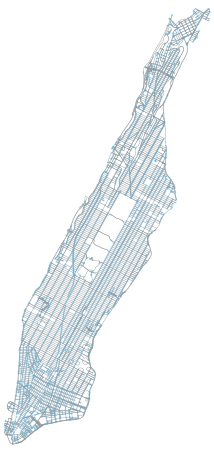
\includegraphics[scale=0.50]{input/images/osmnx.png}
\caption{OSMnx map of manhattan}
\end{figure}
OSMnx: retrieve, construct, analyze, and visualize street networks from OpenStreetMap. OSMnx is a Python package that lets you download spatial geometries and construct, project, visualize, and analyze street networks from OpenStreetMap’s APIs. Users can download and construct walkable, drivable, or bikable urban networks with a single line of Python code, and then easily analyze and visualize them.\\

{\bf Features}
\begin{itemize}
\item Download street networks anywhere in the world with a single line of code
\item Download other infrastructure network types, place polygons, or building footprints as well
\item Download by city name, polygon, bounding box, or point/address + network distance
\item Get drivable, walkable, bikable, or all street networks
\item Visualize the street network as a static image or leaflet web map
\item Simplify and correct the network’s topology to clean and consolidate intersections
\item Save networks to disk as shapefiles or GraphML
\item Conduct topological and spatial analyses to automatically calculate dozens of indicators
\item Calculate and plot shortest-path routes as a static image or leaflet web map
\item Plot figure-ground diagrams of street networks and/or building footprints
\item Download node elevations and calculate edge grades
\item Visualize travel distance and travel time with isoline and isochrone maps
\item Calculate and visualize street bearings and orientations\\

\end{itemize}


{\bf Installation}
\begin{verbatim}
$ sudo apt-get install python-pip python-virtualenv
$ virtualenv venv
$ source venv/bin/activate
$ pip install osmnx
\end{verbatim}

{\bf Usage}
\begin{verbatim}
import osmnx as ox
G = ox.graph_from_place('Punjab, India', network_type='drive')
ox.plot_graph(ox.project_graph(G))
\end{verbatim}


\subsection{NetworkX}

\begin{figure}[h]
\centering 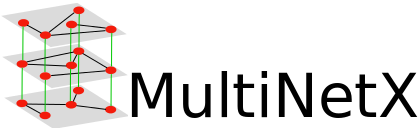
\includegraphics[scale=0.5]{input/images/networkx.png}
\caption{NetworkX logo}
\end{figure}

NetworkX is a Python package for the creation, manipulation, and study of the structure, dynamics, and functions of complex networks.\\

  
{\bf Features}
\begin{itemize}
    \item Data structures for graphs, digraphs, and multigraphs
    \item Many standard graph algorithms
    \item Network structure and analysis measures
    \item Generators for classic graphs, random graphs, and synthetic networks
    \item Nodes can be "anything" (e.g., text, images, XML records)
    \item Edges can hold arbitrary data (e.g., weights, time-series)
    \item Open source 3-clause BSD license
    \item Well tested with over 90\% code coverage
    \item Additional benefits from Python include fast prototyping, easy to teach, and multi-platform
\end{itemize}

{\bf Installation}
\begin{verbatim}
$ sudo apt-get install python-pip python-virtualenv
$ virtualenv venv
$ source venv/bin/activate
$ pip install networkx
\end{verbatim}

{\bf Algorithm}
PageRank computes a ranking of the nodes in the graph G based on the structure of the incoming links. It was originally designed as an algorithm to rank web pages.\\


{\bf Graph types}
\begin{itemize}
\item Undirected Simple
\item Directed Simple
\item With Self-loops
\item With Parallel edges

\end{itemize}


\subsection{GraphFrames}

\\GraphFrames is a package for Apache Spark which provides DataFrame-based Graphs. It provides high-level APIs in Scala, Java, and Python. It aims to provide both the functionality of GraphX and extended functionality taking advantage of Spark DataFrames. This extended functionality includes motif finding, DataFrame-based serialization, and highly expressive graph queries.\\

{\bf What are GraphFrames?}\\
GraphX is to RDDs as GraphFrames are to DataFrames.\\

GraphFrames represent graphs: vertices (e.g., users) and edges (e.g., relationships between users). If you are familiar with GraphX, then GraphFrames will be easy to learn. The key difference is that GraphFrames are based upon Spark DataFrames, rather than RDDs.\\

GraphFrames also provide powerful tools for running queries and standard graph algorithms. With GraphFrames, you can easily search for patterns within graphs, find important vertices, and more. Refer to the User Guide for a full list of queries and algorithms.\\


{\bf creating nodes using pagerank algorithm}
\begin{verbatim}
# Create a Vertex DataFrame with unique ID column "id"
v = sqlContext.createDataFrame([
  ("a", "Alice", 34),
  ("b", "Bob", 36),
  ("c", "Charlie", 30),
], ["id", "name", "age"])

# Create an Edge DataFrame with "src" and "dst" columns
e = sqlContext.createDataFrame([
  ("a", "b", "friend"),
  ("b", "c", "follow"),
  ("c", "b", "follow"),
], ["src", "dst", "relationship"])

# Create a GraphFrame
from graphframes import *
g = GraphFrame(v, e)

# Query: Get in-degree of each vertex.
g.inDegrees.show()

# Query: Count the number of "follow" connections in the graph.
g.edges.filter("relationship = 'follow'").count()

# Run PageRank algorithm, and show results.
results = g.pageRank(resetProbability=0.01, maxIter=20)
results.vertices.select("id", "pagerank").show()
\end{verbatim}

\subsection{Django}
\begin{figure}[h]
	\centering 
\includegraphics[scale=0.2]{input/images/django.png}
	\caption{Django logo}
\end{figure}
\subsubsection{What is Django?}
Django is a high-level Python web framework that enables rapid development of secure and maintainable websites. Built by experienced developers, Django takes care of much of the hassle of web development, so you can focus on writing your app without needing to reinvent the wheel. It is free and open source, has a thriving and active community, great documentation, and many options for free and paid-for support. \\

Django helps you write software that is:
\\
Django follows the "Batteries included" philosophy and provides almost everything developers might want to do "out of the box". Because everything you need is part of the one "product", it all works seamlessly together, follows consistent design principles, and has extensive and up-to-date documentation.\\
Django can be (and has been) used to build almost any type of website — from content management systems and wikis, through to social networks and news sites. It can work with any client-side framework, and can deliver content in almost any format (including HTML, RSS feeds, JSON, XML, etc). The site you are currently reading is based on Django!\\
Django helps developers avoid many common security mistakes by providing a framework that has been engineered to "do the right things" to protect the website automatically. For example, Django provides a secure way to manage user accounts and passwords, avoiding common mistakes like putting session information in cookies where it is vulnerable (instead cookies just contain a key, and the actual data is stored in the database) or directly storing passwords rather than a password hash.\\

A password hash is a fixed-length value created by sending the password through a cryptographic hash function. Django can check if an entered password is correct by running it through the hash function and comparing the output to the stored hash value. However due to the "one-way" nature of the function, even if a stored hash value is compromised it is hard for an attacker to work out the original password.\\

Django enables protection against many vulnerabilities by default, including SQL injection, cross-site scripting, cross-site request forgery and clickjacking (see Website security for more details of such attacks).\\

Django uses a component-based “shared-nothing” architecture (each part of the architecture is independent of the others, and can hence be replaced or changed if needed). Having a clear separation between the different parts means that it can scale for increased traffic by adding hardware at any level: caching servers, database servers, or application servers. Some of the busiest sites have successfully scaled Django to meet their demands (e.g. Instagram and Disqus, to name just two).\\
Django code is written using design principles and patterns that encourage the creation of maintainable and reusable code. In particular, it makes use of the Don't Repeat Yourself (DRY) principle so there is no unnecessary duplication, reducing the amount of code. Django also promotes the grouping of related functionality into reusable "applications" and, at a lower level, groups related code into modules (along the lines of the Model View Controller (MVC) pattern).\\
\subsubsection{Where did it come from?}
Django was initially developed between 2003 and 2005 by a web team who were responsible for creating and maintaining newspaper websites. After creating a number of sites, the team began to factor out and reuse lot of common code and design patterns. This common code evolved into a generic web development framework, which was open-sourced as the "Django" project in July 2005. \\

Django has continued to grow and improve, from its first milestone release (1.0) in September 2008 through to the recently-released version 1.11 (2017). Each release has added new functionality and bug fixes, ranging from support for new types of databases, template engines, and caching, through to the addition of "generic" view functions and classes (which reduce the amount of code that developers have to write for a number of programming tasks). \\
\subsubsection{How popular is Django?}
There isn't any readily-available and definitive measurement of popularity of server-side frameworks (although sites like Hot Frameworks attempt to assess popularity using mechanisms like counting the number of GitHub projects and StackOverflow questions for each platform). A better question is whether Django is "popular enough" to avoid the problems of unpopular platforms. Is it continuing to evolve? Can you get help if you need it? Is there an opportunity for you to get paid work if you learn Django?\\ 

Based on the number of high profile sites that use Django, the number of people contributing to the codebase, and the number of people providing both free and paid for support, then yes, Django is a popular framework!\\

High-profile sites that use Django include: Disqus, Instagram, Knight Foundation, MacArthur Foundation, Mozilla, National Geographic, Open Knowledge Foundation, Pinterest, and Open Stack\\

\subsubsection{Is Django opinionated?}
Web frameworks often refer to themselves as "opinionated" or "unopinionated".\\

Opinionated frameworks are those with opinions about the "right way" to handle any particular task. They often support rapid development in a particular domain (solving problems of a particular type) because the right way to do anything is usually well-understood and well-documented. However they can be less flexible at solving problems outside their main domain, and tend to offer fewer choices for what components and approaches they can use.\\

Unopinionated frameworks, by contrast, have far fewer restrictions on the best way to glue components together to achieve a goal, or even what components should be used. They make it easier for developers to use the most suitable tools to complete a particular task, albeit at the cost that you need to find those components yourself.\\

Django is "somewhat opinionated", and hence delivers the "best of both worlds". It provides a set of components to handle most web development tasks and one (or two) preferred ways to use them. However, Django's decoupled architecture means that you can usually pick and choose from a number of different options, or add support for completely new ones if desired.\\
\subsubsection{What does Django code looks like?}
In a traditional data-driven website, a web application waits for HTTP requests from the web browser (or other client). When a request is received the application works out what is needed based on the URL and possibly information in POST data or GET data. Depending on what is required it may then read or write information from a database or perform other tasks required to satisfy the request. The application will then return a response to the web browser, often dynamically creating an HTML page for the browser to display by inserting the retrieved data into placeholders in an HTML template.\\

Django web applications typically group the code that handles each of these steps into separate files:\\
\begin{figure}[h]
	\centering 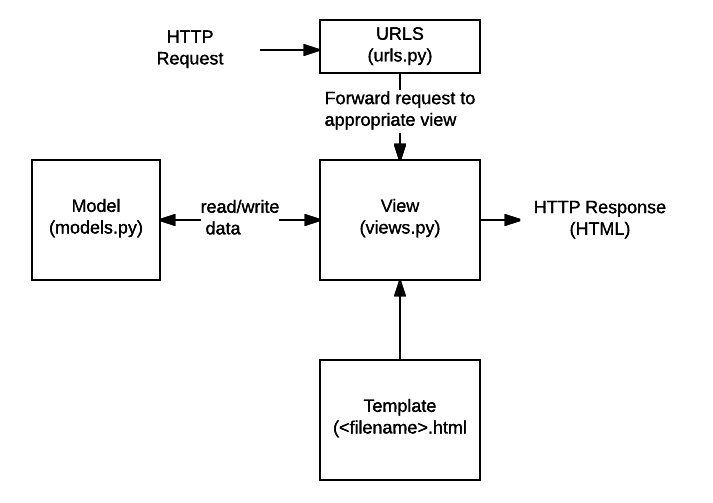
\includegraphics[scale=1]{input/images/django1.png}
	\caption{Django logo}
\end{figure}
\begin{itemize}
	\item URLs: While it is possible to process requests from every single URL via a single function, it is much more maintainable to write a separate view function to handle each resource. A URL mapper is used to redirect HTTP requests to the appropriate view based on the request URL. The URL mapper can also match particular patterns of strings or digits that appear in an URL, and pass these to a view function as data.
	\item View: A view is a request handler function, which receives HTTP requests and returns HTTP responses. Views access the data needed to satisfy requests via models, and delegate the formatting of the response to templates.
	\item Models: Models are Python objects that define the structure of an application's data, and provide mechanisms to manage (add, modify, delete) and query records in the database. 
	\item Templates: A template is a text file defining the structure or layout of a file (such as an HTML page), with placeholders used to represent actual content. A view can dynamically create an HTML page using an HTML template, populating it with data from a model. A template can be used to define the structure of any type of file; it doesn't have to be HTML!
\end{itemize}

\subsection{Apache Spark}
\begin{figure}[h]
	\centering 
\includegraphics[scale=0.2]{input/images/spark.png}
	\caption{Apache Spark logo}
\end{figure}
We are aware that today we have huge data being generated everywhere from various sources. This data is either being stored intentionally in a structured way or getting generated by machines. But data is of no use until we mine it and try to do some kind of analysis on it, in order to come up with actions based on the analysis outcomes. The act of gathering and storing information for eventual analysis is ages old but it had never been based on such a large amount of data, which is there today. There is a specific term for such voluminous data i.e. “Big Data”.

Big data is a term that describes the huge volume of data which can be structured and unstructured or semi-structured. But it’s not the amount of data which is a concern for the organizations since it is just a storage problem which can be easily addressed by the cheap storage available today. It’s what Business get out of the data matters.Big data can be analyzed for insights that lead to better decisions and strategic business moves.

This problem can be solved if we have a framework which not only gives a solution to store all kinds of data (structured, semi-structured or unstructured) but an efficient way of analyzing it according to business needs. One of such framework which is widely used is known as Hadoop. But Hadoop has several limitation (which will be discussed in later sections), because of which Apache Spark was created.

Now we have a solution for our storage and also an efficient way of analyzing data of any size. That means we can make business decisions after analyzing data. But there is another challenge, which is that the decision based on the analysis insight on a huge data might not be relevant after some time. Any decision is useful if we take the action on time, but doing any analysis on huge data takes time, sometimes more than the deadline on which that action had to be performed. So in such cases such insights are of no use because the deadline for action has passed.Processing larger scale of data with Hadoop’s processing framework i.e. MapReduce (MR) is far better than our traditional system but still not good enough for organizations to take all its decision on time, because Hadoop operates on batch processing of data leading to high latency.

Several other shortcomings of Hadoop are:\\

\begin{itemize}
	\item Adherence to its MapReduce programming model
	\item Limited programming language API options
	\item Not a good fit for iterative algorithms like Machine Learning Algorithms
	\item Pipelining of tasks is not easy
\end{itemize}
\subsubsection{What is Spark?}
Apache Spark is an open source data processing framework for performing Big data analytics on distributed computing cluster.

Spark was initially started by Matei Zaharia at UC Berkeley's AMPLab in 2009. It was an academic project in UC Berkley. Initially the idea was to build a cluster management tool, which can support different kind of cluster computing systems. The cluster management tool which was built as a result is Mesos. After Mesos was created, developers built a cluster computing framework on top of it, resulting in the creating of Spark.

Spark was meant to target interactive iterative computations like machine learning. In the year 2013, the spark project was passed on to the Apache Software Foundation.

Spark has several advantages when compared to other big data and MapReduce technologies like Hadoop and Storm. Spark is faster than MaReduce and offers low latency due to reduced disk input and output operation. Spark has the capability of in memory computation and operations, which makes the data processing really fast than other MapReduce.

Unlike Hadoop spark maintains the intermediate results in memory rather than writing every intermediate output to disk. This hugely cuts down the execution time of the operation, resulting in faster execution of task, as more as 100X time a standard MapReduce job. Apache Spark can also hold data onto the disk. When data crosses the threshold of the memory storage it is spilled to the disk. This way spark acts as an extension of MapReduce. Spark doesn’t execute the tasks immediately but maintains a chain of operations as meta-data of the job called DAG. The action on the DAG happens only when an action operation is called on to the transformation DAG. This process is called as lazy evaluation. This allows optimized execution of the queries on Big Data.

Apache Spark has other features, such as:
\\
\begin{itemize}
	\item Supports wide variety of operations, compared to Map and Reduce functions.
	\item Provides concise and consistent APIs in Scala, Java and Python.
	\item Spark is written in Scala Programming Language and runs in JVM.
	\item It currently has support in  the following programming languages to develop applications in Spark:
	\subitem Scala
	\subitem Java
	\subitem Python
	\subitem R
	\item Features interactive shell for Scala and Python. This is not available in Java yet.
	\item It leverages the distributed cluster memory for doing computations for increased speed and data processing.
	Spark enables applications in Hadoop clusters to run up to as much as 100 times faster in memory and 10 times faster even when running in disk.
	It is most suitable for real time decision making with big data.
	\item It runs on top of existing Hadoop cluster and access Hadoop data store (HDFS), it can also process data stored by HBase structure. It can also run without Hadoop with apache Mesos or alone in standalone mode.
	\item Apache Spark can be integrated with various data sources like SQL, NoSQL, S3, HDFS, local file system etc.
	Good fit for iterative tasks like Machine Learning (ML) algorithms.
	\item In addition to Map and Reduce operations, it supports SQL like queries, streaming data, machine learning and data processing in terms of graph.
\end{itemize}
\subsubsection{Hadoop and Spark}
Hadoop as a big data processing technology has proven to be the go to solution for processing large data sets. MapReduce is a great solution for computations, which needs one-pass to complete, but not very efficient for use cases that require multi-pass for computations and algorithms. Each stage in the data processing workflow has one Map and one Reduce phase .To leverage MapReduce solution we need to convert our use case into MapReduce pattern. The Job's output data between each step has to be stored in the file system before the next step can begin. Hence, this approach is slow, due to replication \& disk Input/output operations. Also, Hadoop ecosystem doesn’t have every component to complete a big data use case. It also requires the integration of several other tools for different big data use cases (like Mahout for Machine Learning and Storm for streaming data processing, Flume for log aggregation).

If you want to do an iterative job, you would have to stitch together a sequence of MapReduce jobs and execute them in sequence. Each of those jobs has high-latency, and each depends upon the completion of previous stages. Spark allows programmers to employ complex, multi-step data pipelines using directed acyclic graph (DAG) pattern. It allows in-memory data sharing across DAGs, so that different jobs can work with the same data without going to disk.

Spark can run on top of Hadoop’s distributed file system Hadoop Distributed File System (HDFS) to leverage the distributed replicated storage. Spark can be used along with MapReduce in the same Hadoop cluster or can be used alone as a processing framework. Apache Spark is an alternative to Hadoop MapReduce rather than a replacement of Hadoop. It’s not intended to replace Hadoop but it can regarded as an extension to it. In many use cases MapReduce and Spark can be used together where MapReduce job can be used for batch processing and spark can be used for real-time processing.

\subsubsection{Apache Spark and its components}

SparkContext is an independent process through which spark application runs over a cluster. It gives the handle to the distributed mechanism/cluster so that you may use the resources of the distributed machines in your job. Your application program which will use SparkContext object would be known as driver program. Specifically, to run on a cluster, the SparkContext connects to several types of cluster managers (like Spark’s own standalone cluster manager, apache Mesos or Hadoop's YARN), which allocate resources across applications. Once connected, Spark takes over executors on distributed nodes in the cluster, which are processes in the distributed nodes that run computations and store data for your application. Next, it sends your application code to the executors through SparkContext. Finally tasks are sent to the executors to run and complete it.
\\
\begin{figure}[h]
	\centering 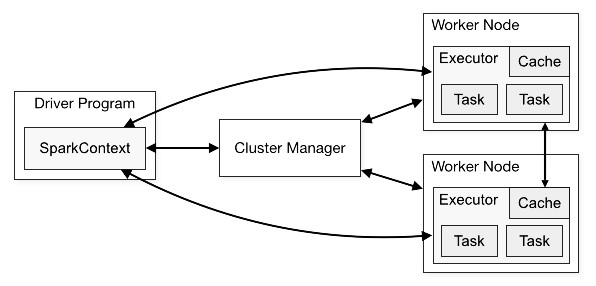
\includegraphics[scale=1]{input/images/spark1.jpg}
	\caption{Spark cluster overview}
	
\end{figure}

\subsubsection{Spark SQL, DataFrames and Datasets}
\begin{itemize} 
\item \textbf{SQL:}
Spark SQL exposes spark APIs to run SQL query like computation on large data. A spark user can perform ad-hoc query and perform near real time ETL on a different types of data like (like JSON, Parquet, Database).

\item \textbf{DataFrames:}
A DataFrame can be considered as a distributed set of data which has been organized into many named columns. It can be compared with a relational table, CSV file or a data frame in R or Python. The DataFrame functionality is made available as API in Scala, Java, Python, and R.

\item \textbf{Dataset:}
A Dataset is a new addition in the list of spark libraries. It is an experimental interface added in Spark 1.6 that tries to provide the benefits of RDDs with the benefits of Spark SQL’s optimized execution engine.

\item \textbf{Spark MLlib And ML:}
MLlib is collective bunch few handy and useful machine learning algorithms and data cleaning and processing approaches which includes classification, clustering, regression, feature extraction, dimensionality reduction, etc. as well as underlying optimization primitives like SGD and BFGS.

\item \textbf{Spark GraphX:}
GraphX is the Spark API for graphs and graph-parallel computation. GraphX enhances the Spark RDD by introducing the Resilient Distributed Property Graph.

A RDD property graph is a directed multi-graph with properties attached with each of its vertex and edge. GraphX has a set of basic operators (like subgraph, joinVertices, aggregateMessages, etc.).Along with operators it has an optimized variant of the Pregel API. GraphX is still under development and many developers are working towards simplification of graph related tasks.

\end{itemize}

\newpage

\section{ Introduction to OSM}
\begin{figure}[ht]
	\centering 
\includegraphics[scale=.50]{input/images/osm-logo.png}
	\caption{OSM foundation}
\end{figure}

  OpenStreetMap (OSM) is a collaborative project to create a free editable map of the world. The creation and growth of OSM has been motivated by restrictions on use or availability of map information across much of the world, and the advent of inexpensive portable satellite navigation devices. OSM is considered a prominent example of volunteered geographic information.\\

Created by Steve Coast in the UK in 2004, it was inspired by the success of Wikipedia and the predominance of proprietary map data in the UK and elsewhere. Since then, it has grown to over 2 million registered users, who can collect data using manual survey, GPS devices, aerial photography, and other free sources. This crowdsourced data is then made available under the Open Database Licence. The site is supported by the OpenStreetMap Foundation, a non-profit organisation registered in England and Wales.\\

Rather than the map itself, the data generated by the OpenStreetMap project is considered its primary output. The data is then available for use in both traditional applications, like its usage by Craigslist, OsmAnd, Geocaching, MapQuest Open, JMP statistical software, and Foursquare to replace Google Maps, and more unusual roles like replacing the default data included with GPS receivers. OpenStreetMap data has been favourably compared with proprietary datasources, though data quality varies worldwide.\\
 
\textbf{Map usage}
Map is available on the following platform.
\begin{itemize}
\item \textbf{Web browser}
    Data provided by the OpenStreetMap project can be viewed in a web browser with JavaScript support via Hypertext Transfer Protocol (HTTP) on its official website.\\
\item \textbf{OsmAnd}
    OsmAnd is free software for Android and iOS mobile devices that can use offline vector data from OSM. It also supports layering OSM vector data with prerendered raster map tiles from OpenStreetMap and other sources.\\
\item \textbf{Maps.me}
    Maps.me is free software for Android and iOS mobile devices that provides offline maps based on OSM data.\\
\item \textbf{GNOME Maps}
    GNOME Maps is a graphical front-end written in JavaScript and introduced in GNOME 3.10. It provides a mechanism to find the user's location with the help of GeoClue, finds directions via GraphHopper and it can deliver a list as answer to queries.\\
\item \textbf{Marble}
    Marble is a KDE virtual globe application which received support for OpenStreetMap.\\
\item \textbf{FoxtrotGPS}
    FoxtrotGPS is a GTK+-based map viewer, that is especially suited to touch input. It is available in the SHR or Debian repositories.\\
\item \textbf{Emerillon}
    Another GTK+-based map viewer.\\

\item The web site OpenStreetMap.org provides a slippy map interface based on the Leaflet JavaScript library (and formerly built on OpenLayers), displaying map tiles rendered by the Mapnik rendering engine, and tiles from other sources including OpenCycleMap.org.\\

\item Custom maps can also be generated from OSM data through various software including Jawg Maps, Mapnik, Mapbox Studio, Mapzen's Tangrams.\\

\item OpenStreetMap maintains lists of online and offline routing engines available, such as the Open Source Routing Machine. OSM data is popular with routing researchers, and is also available to open-source projects and companies to build routing applications (or for any other purpose).\\
\end{itemize}


\newpage

\section{Ubuntu: An open source OS}
\begin{figure}[!ht]
\centering

\includegraphics[width=0.3\textwidth]{input/images/ubuntu.png}                   
\caption{Ubuntu}
\hspace{-1.5em}
\end{figure}
During my training, I also got familiar with a great and open source Operating System, Ubuntu. Firstly, it was quite difficult for a regular MS Windows user to port to Ubuntu. I did all of my project work using this vast operating system. \\
Ubuntu is a Debian-based Linux operating system, with Unity as its default desktop environment. It is based on free software and named after the Southern African philosophy of ubuntu (literally, "human-ness"), which often is translated as "humanity towards others" or "the belief in a universal bond of sharing that connects all humanity".\\
It came under Linux. A kernel normally used by many of the computer persons.You will rarely see a person who is unaware of the term Linux. From perspective of a computer simpleton the one who uses linux mostly shall be having a good knowledge regarding the working of shell,kernel etc.\\

Linux was created by Linus Torvalds. One of a gem of computer scientist who is popular for his OS.\\
Linus was one of the student in Finland and had read a book Operating Systems: Design and Implementation by Andrew S. Tanenbaum.\\
In this book the professor explained about the working of Kernel. To my strange is that he had given the whole source code of his kernel named MINIX in that book. Its really weird but acts as a lucky draw for LInus who took interest in this and with the help of MINIX he created a new OS named Linux. He had told about Andrew in his acknowledgement.\\

Ubuntu's goal is to be secure "out-of-the box". By default user's programs run with low privileges and cannot corrupt the operating system or other user's files. For increased security, the sudo tool is used to assign temporary privileges for performing administrative tasks, which allows the root account to remain locked and helps prevent inexperienced users from inadvertently making catastrophic system changes or opening security holes.\\



\newpage
\section{Introduction to Reveal-js \& Reveal-md}
\begin{figure}[!ht]
\centering

\includegraphics[width=0.3\textwidth]{input/images/rd.jpg}                   
\caption{MD \& JS}
\hspace{-1.5em}
\end{figure}
Reveal-js is one of the framework of Javascript. This can be used for presentations purpose.\\
Now before going to reveal-md lets talk about some fundamental things.\\
What is a Markup language?\\
Markup languages are designed for the processing, definition and presentation of text. The language specifies code for formatting, both the layout and style, within a text file. HTML and Markdown  is an example of a widely known and used markup language.\\
Markdown is a lightweight Markup Language with simple plain text formatting syntax designed so that it can be converted to HTML and many other formats. It is created by  John Gruber. It had '.md' or '.markdown' extention.\\
"Markdown is a text-to-HTML conversion software tool written in Perl for web writers."\\
Moreover, to enable markdown feature of reveal.js, we need reveal-md. The Markdown feature of reveal.js is awesome, and has an easy (and configurable) syntax to separate slides. Use three dashes surrounded by two blank lines.\\
\subsection{Installation of reveal-md}
Installation of reveal-md is a very easy process.
Type the commands in the terminal:\\\\
\emph{
\$ sudo apt-get install npm\\\\
\$ sudo apt-get install nodejs-legacy\\\\
\$ sudo npm install -g reveal-md\\\\}
This will install reveal-md on your pc or laptop.



\newpage

\section{Introduction to \LaTeX}

\LaTeX, I had never heard about this term before doing this project,
but when I came to know about it's features, found it excellent. 
\LaTeX{ is a document markup language and document preparation system for the \TeX{} 
typesetting program. Within the typesetting system, its name is styled 
as \LaTeX.

\begin{figure}[!ht]
\centering
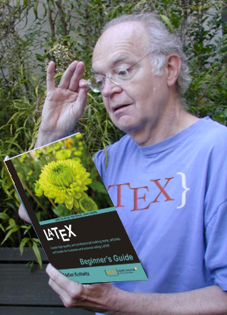
\includegraphics[width=0.3\textwidth]{input/images/donald.png}                   
\caption{Donald Knuth, Inventor Of \TeX{} 
typesetting system}
\hspace{-1.5em}
\end{figure}

Within the typesetting system, its name is styled as \LaTeX. The term 
\LaTeX{} refers only to the language in which documents are written, 
not to the editor used to write those documents. In order to create a 
document in \LaTeX, a .tex file must be created using some form of text 
editor. While most text editors can be used to create a \LaTeX{} document, 
a number of editors have been created specifically for working with \LaTeX.

\LaTeX{} is most widely used by mathematicians, scientists, 
engineers, philosophers, linguists, economists and other scholars in 
academia. As a primary or intermediate format, e.g., translating DocBook 
and other XML-based formats to PDF, \LaTeX{} is used because of the 
high quality of typesetting achievable by \TeX. The typesetting system 
offers programmable desktop publishing features and extensive facilities 
for automating most aspects of typesetting and desktop publishing, 
including numbering and cross-referencing, tables and figures, 
page layout and bibliographies.

\LaTeX{} is intended to provide a high-level language that
accesses the power of \TeX. \LaTeX{} essentially comprises a
collection of \TeX{} macros and a program to process \LaTeX documents. 
Because the \TeX{} formatting commands are very low-level, it is usually 
much simpler for end-users to use \LaTeX{}.

To run LATEX on your own computer, you need  to use a latex distribution. A distribution includes a latex program and (typically) several thousand packages.
\begin{itemize}
  \item  On Windows: MikTEX or TEXLive
   \item On Linux: TEXLive
  \item  On Mac: MacTEX
\end{itemize}
\subsection{Typesetting}
\LaTeX was first developed in 1985 by Leslie Lamport.
In preparing a \LaTeX{} document, the author 
specifies the logical structure using familiar concepts such as 
chapter, section, table, figure, etc., and lets the \LaTeX{} system 
worry about the presentation of these structures. It therefore 
encourages the separation of layout from content while still allowing 
manual typesetting adjustments where needed. 

\begin{verbatim}
\documentclass[12pt]{article}
\usepackage{amsmath}
\title{\LaTeX}
\date{}
\begin{document}
  \maketitle 
  \LaTeX{} is a document preparation system 
  for the \TeX{} typesetting program.
\end{document}
\end{verbatim}

Apart from this lat.pdf; lat.aux, lat.log, lat.pdf files are created by default.\\
\begin{itemize}
\item AUX is a data file format used by Latex
AUX is a data file format used by LaTeX. LaTeX is a macro package which uses TeX typesetting language in its documents. AUX files contain information used for cross-referencing, and is also used to transport information from one compiler run to the next.
\item Some of the compilers are pdftex, Xelatex, Lualatex etc.
\item A log file is usually a flat text file that contains a list of events that happend when a program was running, with one event on each line. Often times errors are recorded in log files.
\item .pdf: The common output format for your document.
Created by pdflatex/ xelatex
\end{itemize}
Happy Texing :)


\newpage

\section{Introduction to Github}
\begin{figure}[!ht]
\centering

\includegraphics[width=0.3\textwidth]{input/images/github}                   
\caption{Github Logo}
\hspace{-1.5em}
\end{figure}
\leavevmode\\
GitHub is a Git repository web-based hosting service which offers all of the functionality of Git as well as adding many of its own features. Unlike Git which is strictly a command-line tool, Github provides a web-based graphical interface and desktop as well as mobile integration. It also provides access control and several collaboration features such as wikis, task management, and bug tracking and feature requests for every project.\\

GitHub offers both paid plans for private repo handle everything from small to very large projects with speed and efficiency. ositories, and free accounts, which are usually used to host open source software projects. As of 2014, Github reports having over 3.4 million users, making it the largest code host in the world.\\

GitHub has become such a staple amongst the open-source development community that many developers have begun considering it a replacement for a conventional resume and some employers require applications to provide a link to and have an active contributing GitHub account in order to qualify for a job.\\

The Git feature that really makes it stand apart from nearly every
other Source Code Management (SCM) out there is its branching model.\\
\\
Git allows and encourages you to have multiple local branches that can
be entirely independent of each other. The creation, merging, and
deletion of those lines of development takes seconds.\\ \\
This means that you can do things like:
\begin{itemize}
\item Frictionless Context Switching.\\ Create a branch to try out an
idea, commit a few times, switch back to where you branched from,
apply a patch, switch back to where you are experimenting, and merge
it in.
\item Role-Based Code lines. \\ Have a branch that always contains only
what goes to production, another that you merge work into for testing,
and several smaller ones for day to day work.
\item Feature Based Work flow. \\ Create new branches for each new
feature you're working on so you can seamlessly switch back and forth
between them, then delete each branch when that feature gets merged
into your main line.
\item Disposable Experimentation.\\  Create a branch to experiment in,
realize it's not going to work, and just delete it - abandoning the
work—with nobody else ever seeing it (even if you've pushed other
branches in the meantime).
\end{itemize}
Notably, when you push to a remote repository, you do not have to push
all of your branches. You can choose to share just one of your
branches, a few of them, or all of them. This tends to free people to
try new ideas without worrying about having to plan how and when they
are going to merge it in or share it with others.\\ \\
There are ways to accomplish some of this with other systems, but the
work involved is much more difficult and error-prone. Git makes this
process incredibly easy and it changes the way most developers work
when they learn it.

\subsection{What is Git?}
\begin{figure}[!ht]
\centering

\includegraphics[width=0.3\textwidth]{input/images/git}                   
\caption{Git Logo}
\hspace{-1.5em}
\end{figure}
Git is a distributed revision control and source code management (SCM) system with an emphasis on speed, data integrity, and support for distributed, non-linear workflows. Git was initially designed and developed by Linus Torvalds for Linux kernel development in 2005, and has since become the most widely adopted version control system for software development.\\

As with most other distributed revision control systems, and unlike most client–server systems, every Git working directory is a full-fledged repository with complete history and full version-tracking capabilities, independent of network access or a central server. Like the Linux kernel, Git is free and open source software distributed under the terms of the GNU General Public License version 2 to handle everything from small to very large projects with speed and efficiency.\\

Git is easy to learn and has a tiny footprint with lightning fast performance. It outclasses SCM tools like Subversion, CVS, Perforce, and ClearCase with features like cheap local branching, convenient staging areas, and multiple workflows.\\

\subsection{Installation of Git}

Installation of git is a very easy process.
The current git version is: 2.0.4.
Type the commands in the terminal:\\\\
\emph{
\$ sudo apt-get update\\\\
\$ sudo apt-get install git\\\\}
This will install the git on your pc or laptop.

\subsection{Various Git Commands}

Git is the open source distributed version control system that facilitates GitHub activities on your laptop or desktop. The commonly used Git command line instructions are:-\\

\subsubsection{Create Repositories}
Start a new repository or obtain from an exiting URL

\begin{description}

\item [\$ git init [ project-name]]\\
Creates a new local repository with the specified name
\item [\$ git clone [url]]\\
Downloads a project and its entire version history\\

\end{description}


\subsubsection{Make Changes}
Review edits and craft a commit transaction

\begin{description}

\item [\$ git status] \leavevmode \\
Lists all new or modified files to be committed.

\item [\$ git add [file]]\\
Snapshots the file in preparation for versioning.

\item [\$ git commit -m "[descriptive message]"]\\
Records file snapshots permanently in version history.\\

\end{description}


\subsubsection{Group Changes}
Name a series of commits and combine completed efforts

\begin{description}

\item [\$ git branch] \leavevmode \\
Lists all local branches in the current repository.

\item [\$ git branch [branch-name]]\\
Creates a new branch.

\item [\$ git checkout [branch-name]]\\
Switches to the specified branch and updates the working directory.\\

\item [\$ git branch -d [branch-name]]\\
Deletes the specified branch.\\

\end{description}


\subsubsection{Synchronize Changes}
Register a repository bookmark and exchange version history.

\begin{description}

\item [\$ git push [alias][branch]]\\
Uploads all local branch commits to GitHub.

\item [\$ git pull] \leavevmode \\
Downloads bookmark history and incorporates changes.

\end{description}








\chapter{Experimental Results and Comparison}

\section{Experimental Results}
I had tried my project on different server also i.e Experimental Server here. I had tried it on both ubuntu 14.04 and 15.10. It works fine on both versions.\\
Below is one of the experimental result.\\
\begin{figure}[!ht]
	\centering
	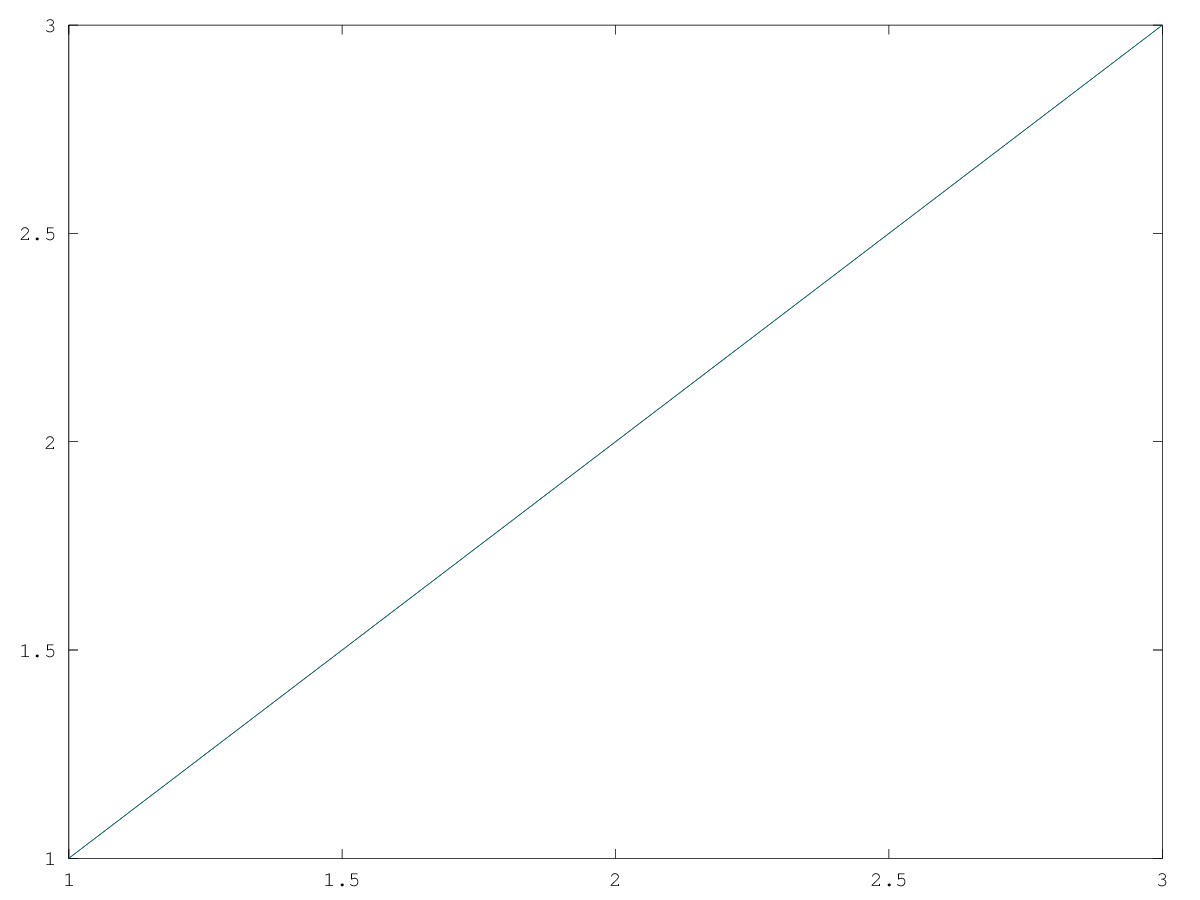
\includegraphics[width=0.7\textwidth]{input/images/plot1.png}                
	\caption{Graph Plotted}
	\hspace{-1.5em}
\end{figure}\\
You may refer to my blogs also for detailed information.\\
Here is the url: \\
https://deepti96.wordpress.com/ \\\\
The interface of Web-Octave looks like this but can be changed using CSS file.
\begin{figure}[!ht]
	\centering
	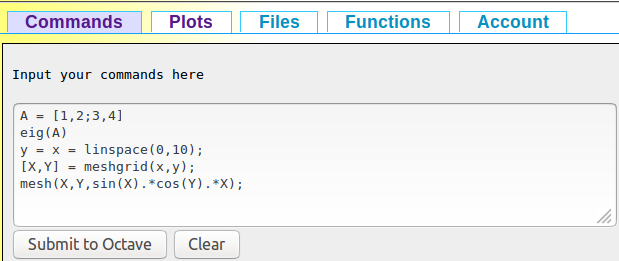
\includegraphics[width=0.7\textwidth]{input/images/p.png}                
	\caption{Code}
	\hspace{-1.5em}
\end{figure}\\\\
Output of above code is: \\
\begin{figure}[!ht]
	\centering
	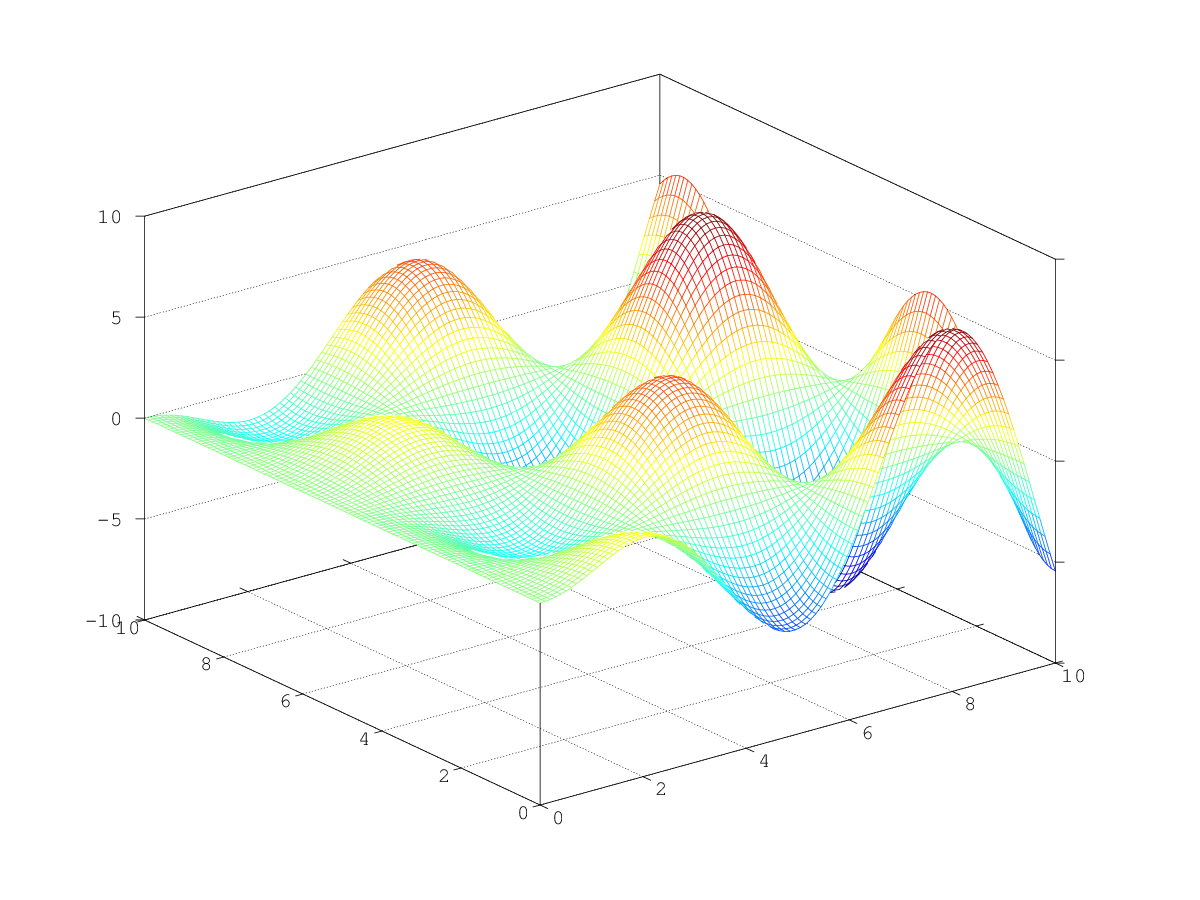
\includegraphics[width=0.7\textwidth]{input/images/plot2.png}                
	\caption{Output}
	\hspace{-1.5em}
\end{figure}\\
\subsection{Testing}
Testing a program consists of providing the program with a set of test inputs (or test cases) and
observing if the program behaves as expected. If the program fails to behave as expected, then the
conditions under which failure occurs are noted for later debugging and correction. \\
This software had been taken through rigorous test to fully found potential causes of error and system failure
and full focus have been given to cover all possible exceptions that can 
occur and cause failure of the software.\\
As this software is based on intensive background process it have been taken care that 
if correct input and email address are given then processing of user job can even continue or a least automatically 
restart even after server shuts down or even crash.

\begin{table}[h]
\centering
\begin{tabular}{ ||c|c|| }
\hline
 \multicolumn{2}{||c||}{Overview of Octave versions} \\
 \hline
 Date & Publication Title \\ [0.5ex] 
 \hline \hline
	September 1999 & Octave framework 1.0 \\ \hline
	September 2001 & Octave framework 2.0 \\ \hline
	December 2001 & Octave criteria 2.0\\ \hline
	September 2003 & Octave-S v0.9 \\ \hline
	March 2005 & Octave-S v1.0 \\ \hline
	June 2007 & Octave 3.x\\ \hline
        March 2016 &  Octave 4.0.1        \\ \hline
	July 2016 & Octave 4.0.3 \\ [1ex]
 \hline
\end{tabular}
\caption{Octave Release}
\label{table2}
\end{table}

\begin{table}[h]
\centering
\resizebox{\textwidth}{!}{\begin{tabular}{ |c|c|c|c| }
\hline
 \multicolumn{4}{|c|}{Test cases for main page(index.html) } \\[0.5ex]
 \hline
 Input & Desired Output & Actual Output & Status \\ [0.5ex] 
 \hline \hline
 Inputs range exceeds & Alert user,Don't proceed & Alert user,Don't proceed. & Pass\\ \hline
 Incomplete Command & Alert user about range. Don't proceed & Alert user about range. Don't proceed & Pass\\ \hline
 PNG selected: No & Error & Don't proceed & Pass\\ \hline
 Session: Yes & Show email field after Submit & Show email field after Submit & Pass\\ \hline
 Help pressed  & Show Detailed user help & Show Detailed user help  & Pass\\ \hline
 
\end{tabular}}
\caption{Computational Analysis}
\label{table3}
\end{table}
\begin{table}[h]
\centering
\resizebox{\textwidth}{!}{
\begin{tabular}{ |c|c|c|c| }
\hline
 \multicolumn{4}{|c|}{Test cases for possible source of problems } \\[0.5ex]
 \hline
  Input & Desired Output & Actual Output & Status \\ [0.5ex] 
 \hline \hline 
 URL refreshed & Send to homepage & Send to homepage & Pass\\ \hline
 server stops or rebooted & Start processing interrupted requests & Start processing interrupted requests & Pass\\ \hline
\end{tabular}}



\caption{Test case (general)}
\label{table}
\end{table}
 
 
 


\chapter{Conclusion,Summary and Future Scope}

\section{Future Scope}
To analyze OSM data using NetworkX is ideal for small data sets but when data becomes large this approach becomes vague and at that point we need a new technology which incorporates Big Data and such technologies are Hadoop, Apache Spark and various others, but Hadoop and Apache Spark are the most popular, Apache spark is 100 times faster than mapreduce pardigm in Hadoop, Graphframes API is used as it supports Python and Larger datasets can be analyzed in future of this project.\\
The analyzed data can be used for various purposes like urban planning and improving quality of traffic to make roads safer and better. Construction of new roads or starting metro or bus services might benifit this anlysis and provide good quality service to the commuters.





\section{Technical and Managerial Lesson Learnt}
I learned a lot by doing this project . During this period I got to learn a vast 
number of technologies. These are listed below :
\begin{itemize}
\item {\bf{Operating system}}: Ubuntu
\item {\bf{Languages used}}: PHP, HTML, CSS, MySQL
\item {\bf{Framework}}: Reveal.js, Reveal-md
\item {\bf{Typesetting}}: LaTex
\item {\bf{Other Learnings}}:  Wordpress, Markdown

\end{itemize}

% Edit this file%
So during this project I learned all the above things. Above all I got to know 
how Softwares are developed from the scratch. Planning, designing, developing code, 
working in a team, testing etc. These are all very precious things I got to learn 
during this period.  




\begin{thebibliography}{9}
\bibitem{} Ntwx, https://github.com/AFCgooner29/Majorproject
\bibitem{} \LaTeX{} Beginner's Guide By Stefan Kottwitz 
\bibitem{} Blog Followed, http://geoffboeing.com/
\bibitem{} Our Github Profile, https://github.com/AFCgooner29/ , https://github.com/singh1114/
\bibitem{} Online Sources , https://graphframes.github.io/
\bibitem{} OSMNx Blog, http://geoffboeing.com/
\bibitem{} https://spark.apache.org/
\bibitem{} https://www.djangoproject.com/


\end{thebibliography}



\end{document}

